\section{Preliminaries}
    \subsection{Lattice-Based Cryptography} \marginnote{YWW}
    Lattice-based cryptography is compelling for the following reasons:
    \begin{itemize}
        \item \textbf{Post-quantum security:} Many lattice-based problems are conjectured to be hard for both classical and quantum adversaries, making lattice-based cryptography one of the candidates in NIST's post-quantum cryptography standardization process \cite{nist_pqc}.
        \item \textbf{Enables advanced cryptographic schemes:} Lattice-based cryptography provides a rich algebraic structure, thereby enabling the construction of advanced cryptographic schemes, e.g., fully homomorphic encryption \cite{BGV} \cite{bfv1} \cite{bfv2}, homomorphic signatures \cite{hsig}, and functional encryption \cite{FE}. Until very recently, lattice-based cryptography
        provided the only such realizations of these advanced schemes.
        \item \textbf{Security based on worst case hardness:} Cryptography typically based the security on average case hardness, which is a stronger requirement compared with average case hardness. However, lattice-based cryptography allows us to base security on average case hardness: Some results \cite{av1} \cite{av2} \cite{av3} \cite{av4} \cite{av5} show that certain problems (e.g. LWE, SIS problem, and their ring and module variants) are hard on average case, provided that the closely related lattice problems, e.g. approximate SVP, SIVP, are hard in the worst case. Thus, schemes based on these problems are secure unless all instances of those lattice problems are solvable in polynomial time.
    \end{itemize}
    \subsection{Learning with Errors (LWE) Problem} \marginnote{YWW}
    The Learning with Errors (LWE) problem is a cornerstone of modern lattice-based cryptography. It was introduced by Regev \cite{av1} and its hardness is based on certain assumptions regarding the worst-case hardness of standard lattice problems such as GAPSVP (the decision version of the shortest vector problem) and SIVP (the shortest independent vectors problem) \cite{Reg05, Pei09a}.
    
    \begin{definition}[LWE Distribution]
        Let $n \ge 1$ be the security parameter (dimension), $q \ge 2$ be a modulus, and $\chi$ be an error distribution over $\mathbb{Z}_q$. For a secret vector $\mathbf{s} \in \mathbb{Z}_q^n$, the LWE distribution $A_{\mathbf{s}, \chi}$ over $\mathbb{Z}_q^n \times \mathbb{Z}_q$ is sampled by choosing a vector $\mathbf{a} \in \mathbb{Z}_q^n$ uniformly at random, sampling an error $e$ from the distribution $\chi$, and outputting the pair $(\mathbf{a}, b = \langle \mathbf{a}, \mathbf{s} \rangle + e) \in \mathbb{Z}_q^n \times \mathbb{Z}_q$.
    \end{definition}
    \noindent The LWE problem has two primary forms: the search version and the decision version. The goal of the search problem is to recover the secret vector from given LWE samples. The decision problem, on the other hand, is to distinguish LWE samples from uniformly random ones. These problems are parameterized by the number of samples, $m$, which we usually take to be large enough that the secret is uniquely defined with high probability.
    \begin{definition}[Search LWE Problem]
    Given $m$ independent samples $(\mathbf{a}_i, b_i) \in \mathbb{Z}_q^n \times \mathbb{Z}_q$ drawn from $A_{\mathbf{s},\chi}$ for a uniformly random secret $\mathbf{s} \in \mathbb{Z}_q^n$ (fixed for all samples), the goal of the \textbf{search LWE problem}, denoted $\text{Search-LWE}_{n,q,\chi,m}$, is to find $\mathbf{s}$.
    \end{definition}

        \begin{definition}[Decisional LWE Problem]
    Given $m$ independent samples $(\mathbf{a}_i, b_i) \in \mathbb{Z}_q^n \times \mathbb{Z}_q$, where every sample is distributed according to either: (1) $A_{\mathbf{s},\chi}$ for a uniformly random $\mathbf{s} \in \mathbb{Z}_q^n$ (fixed for all samples), or (2) the uniform distribution, the goal of the \textbf{decisional LWE problem}, denoted $\text{Decision-LWE}_{n,q,\chi,m}$, is to distinguish which is the case with non-negligible advantage.
    \end{definition}

    \subsection{Ring Learning with Errors (RLWE) Problem} \marginnote{YWW}
    The Ring Learning with Errors (RLWE) problem, introduced by Lyubashevsky, Peikert, and Regev \cite{idealLatticeRLWE}, is an algebraic variant of LWE that provides significant efficiency improvements. Instead of working with vectors of integers, RLWE operates over polynomial rings, which allows for more compact ciphertexts and faster computations. The security of many modern cryptographic schemes, e.g. the fully homomorphic encryption scheme used in this lab (CKKS scheme \cite{cheon2017homomorphic}), is based on the hardness of the RLWE problem.
    \begin{definition}[Cyclotomic Ring]
    Let $\Phi_M(X)$ be the $M$-th cyclotomic polynomial of degree $N$. Let $\mathcal{R} = \mathbb{Z}[X]/\Phi_M(X)$ be the integer ring and write $\mathcal{R}/q \mathcal{R}$ as the residue ring of $\mathcal{R}$ modulo an integer $q$.\\
    In the CKKS scheme, polynomial with a power-of-two-degree is used, and $M$ is always twice that degree, i.e. the ring used in CKKS scheme is $\mathcal{R} = \mathbb{Z}[X]/(X^N + 1)$ and $N = M/2$.\\
    For an integer polynomial $a \in \mathcal{R} = \mathbb{Z}[X]/\Phi_M(X)$, the canonical embedding $CE(a)$ is $(a(\zeta_{M}^j)) \in \mathbb{C}^N$ where $0 < j < M$, $j \in \mathbb{Z}_M^\times$ and $\zeta_M = e^{2\pi i / M}$ is the primitive $M$th root of unity.
    \end{definition}
    
    \begin{definition}[Gaussian Distribution]
    For a real number $r$, we define the the Gaussian function as $\rho _r = \text{exp}(-\pi ||\mathbf{z}||^2 /r^2)$, where $||\mathbf{z}||$ is the $L_{2}$ norm of the vector $\mathbf{z}$.
    As a discrete Gaussian distribution is usually used as the RLWE error distribution, the continuous Gaussian distribution $\Psi_\mathbf{r}$ has to be discretized by a rounding function to the nearest integer, i.e. $\lfloor \Psi_\mathbf{r} \rceil$.
    \end{definition}

    \begin{definition}[RLWE Distribution]
Here, we define the (decisional) RLWE distribution as follows. We use the dual  $\mathcal{R}^{\lor} = N^{-1} \cdot \mathcal{R}$ as the fractional ideal of $\mathcal{R}$ and $\mathcal{R}^\lor_q = \mathcal{R}^\lor/q\mathcal{R}^\lor$. For a secret $s \in \mathcal{R}_q^\lor$, let $q \geq 2$ be the modulus,  $\mathbf{r} \in (\mathbb{R}_{>0}) ^N$ and an error distribution $\chi := \lfloor \Psi_\mathbf{r} \rceil_{\mathbb{R}^{\lor}}$, a RLWE distribution $A_{N,q,\chi}(s)$ over $\mathcal{R}_q \times \mathcal{R}_q^\lor$ is sampled by choosing $a \leftarrow \mathcal{R}_q$ uniformly at random, $e \leftarrow \chi$, and output an RLWE instance as $(a, a \cdot s + e) \in \mathcal{R}_q \times \mathcal{R}_q^\lor$\footnote{Note that the form of RLWE sample is sometimes written as $(a, a \cdot s + e) \in \mathcal{R}_q \times \mathcal{R}_q^$. The RLWE problems in these two forms are entirely equivalent in terms of computation, but it turns out that  $\mathcal{R}_q \times \mathcal{R}_q^\lor$ form is the right definition for hardness proof and cryptographic applications when using a (nearly) spherical error $e$ \cite {idealLatticeRLWE} \cite{toolkitRLWE}. To obtain this form of RLWE instance, $s, (a \cdot s + e) \in \mathcal{R}_q^\lor$ can be transformed by multiplying them by a tweak factor $t$, such that $ts, (a \cdot ts + te) \in \mathcal{R}_q$ and $(a, a \cdot ts + te) \in \mathcal{R}_q \times \mathcal{R}_q^$. As CKKS scheme uses a power-of-two cyclotomic ring, the dual is $\mathcal{R}^{\lor} = N^{-1} \cdot \mathcal{R}$. Thus the tweak factor for $s$ and $e$ is just $N$.}.
\end{definition}
\begin{definition}[Search RLWE Problem]
The \textbf{search RLWE problem} is to recover the secret $s$ from a given set of samples from the RLWE distribution $A_{N,q,\chi}(s)$.
\end{definition}
\begin{definition}[Decisional RLWE Problem]
The decisional RLWE problem is to distinguish between the samples drawn from the RLWE distribution $A_{N,q,\chi}(s)$ and the samples drawn uniformly at random from the distribution $\mathcal{R}_q \times \mathcal{R}_q^\lor$, with non-negligible probability.
\end{definition}

\subsection{Module Learning with Errors (MLWE) Problem} \marginnote{YWW}
The Module Learning with Errors (MLWE) problem \cite{BGV} \cite{mlwe} is a generalization of the LWE and RLWE problem. It offers a flexible trade-off between the efficiency of RLWE and the generality of LWE. Instead of working with single polynomials in a ring $\mathcal{R}$, MLWE operates on modules over the ring $\mathcal{R}$, which are essentially vectors of ring elements. Because of its flexibility, its concrete-security/efficiency trade-off is highly tunable, and Kyber and Dilithium \cite{kyber, dilithium}, the KEM and signature scheme in NIST PQC standard, are based on MLWE.
\begin{definition}[MLWE Distribution]
Let $\mathcal{R}_q$ be a polynomial ring modulo $q$ (e.g. $\mathcal{R}_q = \mathbb{Z}_q[X]/(X^d + 1)$), $d \ge 1$ be the degree of the polynomial, $k$ be the rank of the module, and $\chi$ be an error distribution over $\mathcal{R}_q$. For a secret vector $\mathbf{s} \in \mathcal{R}_q^k$, the MLWE distribution $A_{\mathbf{s}, \chi}$ is sampled by choosing a vector $\mathbf{a} \in \mathcal{R}_q^k$ uniformly at random, sampling an error $e \leftarrow \chi$, and outputting the pair $(\mathbf{a}, b = \langle \mathbf{a}, \mathbf{s} \rangle + e) \in \mathcal{R}_q^k \times \mathcal{R}_q$.
\end{definition}
\noindent Using $\mathbb{Z}_q$ as the $\mathcal{R}_q$ in the MLWE definition obtains the plain LWE definition. On the other hand, setting $k=1$ obtains the RLWE definition.
\begin{definition}[Search MLWE Problem]
Given a set of samples from the MLWE distribution, the \textbf{search MLWE problem} is to recover the secret vector $\mathbf{s}$.
\end{definition}

\begin{definition}[Decisional MLWE Problem]
The \textbf{decisional MLWE problem} is to distinguish between samples from the MLWE distribution and uniformly random samples from $\mathcal{R}_q^k \times \mathcal{R}_q$.
\end{definition}

    \subsection{Fully Homomorphic Encryption and Bootstrapping} \marginnote{YWW}
    Fully homomorphic encryption is an encryption scheme that enables computation on encrypted data and produces encrypted results matching those of plaintext computations, without needing to decrypt the data to know the decryption key. More precisely, one can take a set of encrypted message \textsf{Enc}$(x_1),...,$\textsf{Enc}$(x_n)$ and  homomorphically compute a function on this set, i.e.  produce an encryption of the function of them, that is, \textsf{Enc}$(f(x_1,...,x_n))$. The homomorphic computation is correct, i.e. 
    \[
    \textsf{Dec}_{sk}(\textsf{Enc}_{pk}(f(x_1,...,x_n))) = f(x_1,...,x_n).
    \]
    Homomorphic encryption schemes built from LWE usually have a problem of error growth from homomorphic computations, which makes the scheme being not able to compute functions correctly after the error grows to a certain size. These schemes can only homomorphically evaluate a circuit of a bounded depth, and they are usually called `somewhat homomorphic' or `leveled homomorphic'.\\
    A concept called `bootstrapping' proposed by Gentry \cite{bootstrapping} allows us to reduce the error rate of a ciphertext, thus enables homomorphic computation with unbounded depth. Such an encryption scheme with unbounded depth is called fully homomorphic encryption. Suppose we have a ciphertext $C$ of the plaintext $m$, where its error rate is too large for a further homomorphic operation. The idea behind bootstrapping is to encrypt the secret key, i.e. $\textsf{Enc}(sk)$, then homomorphically evaluate the decryption function on $C$ and $\textsf{Enc}(sk)$. Thus, the homomorphic decryption function $\textsf{Dec}_{HE}$ will produce a `refreshed' ciphertext $C'$, which is the encryption of $m$ with a lower error rate:
    \[
    \textsf{Dec}_{HE}(\textsf{Enc}(sk), C) = C', \textsf{Dec}(C') = m.
    \]
    \subsection{Cheon-Kim-Kim-Song homomorphic encryption scheme} \marginnote{YWW}
    The CKKS scheme is a fully homomorphic encryption scheme for approximate arithmetic, which supports approximate addition and multiplication on real numbers with unbounded depth. Its security is based on the hardness to solve the ring learning with errors problem (RLWE), and the decryption of this scheme results in a small error on data, which is acceptable for some real world applications.\\
    \\
    \textbf{Batching and plaintext encoding.} 
    The idea of batching in FHE scheme is to batch multiple plaintexts into a single ciphertext, which allows us to perform homomorphic computation efficiently with parallel computation. As the CKKS scheme relies on RLWE, the batched vectors must be encoded into polynomials contained in an appropriate cyclotomic ring. The idea of encoding and decoding is to use the canonical embedding, e.g.\@{} a plaintext vector $\mathbf{z} \in \mathbb{C}^{N/2}$ is encoded as a polynomial $m(X) \in \mathbb{Z}[X]/(X^N +1)$ by the inverse of canonical embedding and vice versa. \\
    More precisely, the image of the canonical embedding is in the subring $\mathbb{H} = \{(z_j)_{j \in \mathbb{Z}_M^{\times}}: z_j = \overline{z_{-j}} \}$ of  $\mathbb{C}^N$. As half of the elements in $\mathbb{H}$ are conjugate to the other half, the plaintext vectors $\mathbf{z}$ are in $\mathbb{C}^{N/2}$. To project from $\mathbb{C}^{N}$ to $\mathbb{C}^{N/2}$, a projection $\pi$ is defined by $(z_j)_{j \in \mathbb{Z}_M^{\times}} \mapsto (z_j)_{j \in T}$ where $T$ is a multiplicative subgroup of $\mathbb{Z}_M^{\times}$ satisfying $\mathbb{Z}_M^{\times} / T = \{ \pm 1\}$.\\
    In the encoding algorithm, we first need to expand vector $\mathbf{z} \in \mathbb{C}^{N/2}$ to $\mathbb{C}^{N}$ by using $\pi^{-1}$.  As $CE(\mathcal{R})$ is countable but $\mathbb{H}$ is isomorphic to $\mathbb{C}^{N/2}$ (defined by $\pi$) and uncountable, $\pi^{-1}(\mathbf{z})$ may not be in  $CE(\mathcal{R})$. Thus we need to discretize $\pi^{-1}(\mathbf{z})$ by the coordinate-wise randomized rounding (written as $\lfloor\,\,  \rceil_{CE(\mathcal{R})}$) \cite{toolkitRLWE}. \\
    As rounding in encoding process may destroy some significant figures, we need to multiply the plaintext by a scaling factor $\Delta$ before encoding, and divide it by $\Delta^{-1}$ in the decoding algorithm. \\
    The full encoding and decoding algorithm are defined as follows: 
    \begin{itemize}
    \item Encoding: a vector $\mathbf{z} \in \mathbb{C}^{N/2}$ is taken as input. We first expand it to $\pi^{-1}(\mathbf{z}) \in \mathbb{H}$, then multiply it by the scaling factor $\Delta$, followed by the rounding function. Finally, apply the inverse of canonical embedding $CE^{-1}$. The resulting polynomial is$$m(X) = CE^{-1}(\lfloor\Delta\cdot\pi^{-1}(\mathbf{z})\rceil_{CE(\mathcal{R})} \in \mathcal{R}$$
    \item Decoding: a polynomial $m \in \mathcal{R}$ is taken as input. The resulting vector is $$z = \pi \circ CE(\Delta^{-1}\cdot m) \in \mathbb{C}^{N/2}$$
    \end{itemize}
    \textbf{Encryption and decryption.} In the CKKS scheme, the encryption of a plaintext $m$ outputs $(c_0, c_1) = (-a \cdot s + e + m, a) \mod q$, and the decryption of a ciphertext is $\textsf{Dec}_s(c_0, c_1) = c_0 + c_1 \cdot s = (-a \cdot s + e + m) + a \cdot s = m + e \mod q$.\\
    \\
    \textbf{Bootstrapping.} As the decryption algorithm consists of a modular reduction, the bootstrapping of CKKS scheme thus includes a homomorphic modular reduction. Since CKKS scheme is infeasible to do homomorphic modular reduction, Cheon et al. \cite{10.1007/978-3-319-78381-9_14} proposed a bootstrapping for CKKS scheme where the  decryption formula is approximated by an approximate polynomial of a scaled sine function. A trigonometric function is a good approximation of modular reduction because it is the identity near zero and periodic with period $q$. \\
    \\
    \subsection{Logistic Regression} \marginnote{YWW}
    Logistic regression is a common supervised machine learning model mainly for two-class classification. Consider an observation $x$ with features $[x_1, x_2,...,x_n]$ and it can be classified as one of the two classes, the main idea of logistic regression is to apply the learned parameters (weights and bias) to the features, then uses the logistic sigmoid function as the classifier to classifies that observation as one of the two classes (A real world example can be a spam filter classifying an email as `spam' or `not spam'). Weights $w_i$ are real numbers which represent how important the features $x_i$ is to the classification. \@{}Bias $b$, also called intercept, is another real number which is added to the weighted features. Applying weights and bias to the features means:
    \[
    \left(\sum_{i = 1}^{N}w_ix_i \right) + b
    \]
    We simplify the above notation with $w_0 = b$ and $x_0 = 1$:
    \[
    \left(\sum_{i = 0}^{N}w_ix_i \right)
    \]
    Logistic sigmoid function is used as the classifier of logistic regression. The function has the form
    \[
    \sigma(a) = \frac{1}{1 + \exp(-a)}
    \]
    and always maps to a range of $[0, 1]$, which can be used as the probability of an observation being classified as a certain class. The term `sigmoid' means S-shaped, as you can see in figure \ref{fig:LR}. This type of function is usually called `squashing function' because it maps the whole real axis into a finite interval. 
       \begin{figure}[ht]
        \centering
        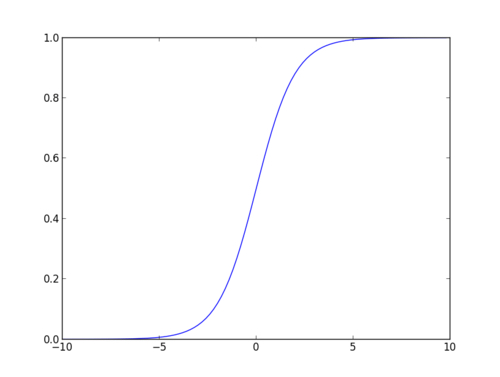
\includegraphics[width=0.5\linewidth]{images/LR.jpg}
        \caption{Plot of the logistic sigmoid function}
        \label{fig:LR}
    \end{figure} 
    As CKKS scheme can only evaluate polynomial function, the logistic sigmoid function can only be approximated by a specific polynomial. Refer to section 3.1 for details.\\
    \\
    To use the sigmoid function as the classifier, we apply the function to the weighted features. Suppose the two classes of our data set are $\textcal{C}_0, \textcal{C}_1$, $\mathbf{x}$ is the feature vector of an observation and $\mathbf{w}$ is the weight vector, the probability of that observation classified as  $\textcal{C}_0$ is
    \[
    prob.(\text{label} = \textcal{C}_0 | \mathbf{x}) = \sigma(\mathbf{w}^T\mathbf{x}) = \frac{1}{1 + \exp(-\mathbf{w}^T\mathbf{x})}
    \]
    and the probability for the other class is 
     \[
    prob.(\text{label} = \textcal{C}_1 | \mathbf{x}) = 1 - \sigma(\mathbf{w}^T\mathbf{x}) = 1 - \frac{1}{1 + \exp(-\mathbf{w}^T\mathbf{x})} = \frac{\exp(-\mathbf{w}^T\mathbf{x})}{1 + \exp(-\mathbf{w}^T\mathbf{x})}
    \]
    As the sigmoid funtion has the property:
    \[
    1 - \sigma(a) = \sigma(-a)
    \]
    we can express $prob.(\text{label} = \textcal{C}_1 | \mathbf{x})$ as $\sigma(-(\mathbf{w}^T\mathbf{x}))$.\\
    \\
    To optimise the accuracy of the classifier, logistic regression learns the weights and bias from the training data set at training phase, such that the classified classes are as close to the true classes as possible. We use gradient descent as our optimisation algorithm.
    \subsection{Optimisation Methods for Logistic Regression with CKKS} \marginnote{VTN}
   To optimise the accuracy of the model, nonlinear optimization methods are needed to estimate the regression parameters, i.e. weights and bias. The most well-known cost function optimization approaches in logistic regression are the Newton-Raphson method and the gradient descent method. Since matrix inversion is a must when using the Newton-Raphson method and the CKKS scheme does not support that feature, we put the Newton-Raphson method aside and consider the gradient descent method to train the encrypted datasets. Fortunately, the gradient descent method does not need matrix inversion and any division operations, as a result it is suitable for training the CKKS encrypted data.\\
   \subsection{Gradient Descent} \marginnote{YWW}
    Gradient descent is a common optimisation algorithm in machine learning to learn the model parameters. The main idea is to define a cost function (or error function) for the classifier, then iteratively update the parameters to go to the negative direction of the gradient of the error function at the current point until it goes to the local minimum.\\
       \begin{figure}[ht]
        \centering
        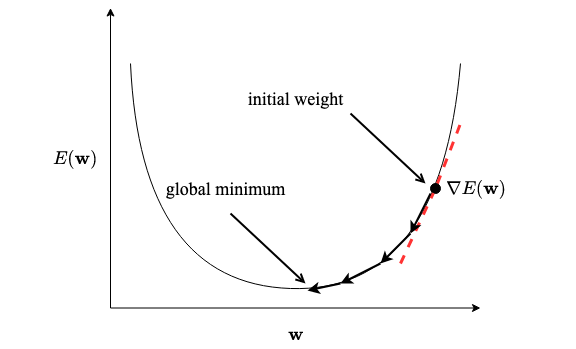
\includegraphics[width=0.8\linewidth]{images/gradient descent.png}
        \caption{Example of gradient descent which iteratively goes to the negative direction of the gradient until it reaches the local minimum (also global minimum in this example).}
        \label{fig:GD}
    \end{figure} 
    \\
    For a training data set $\{X, T\}$ with $N$ data points, we denote $x_i$ as the features of a single data point $i = 1,...,N$ and $t_i \in \{0, 1 \}$ is the true class. As the true classes are binary, the data set is a Bernoulli distribution. The probability or likelihood for a single data point is:
    \[
    prob.(t_i | x_i) = y_i^{t_i} (1 - y_i)^{1 - t_i}
    \]
    and the likelihood function for the data set is:
    \[
    prob.(T | X) = {\displaystyle \prod_{i=1}^{N} y_i^{t_i}(1 - y_i)^{1 - t_i}}
    \]
    where $y_i = \sigma(\mathbf{w}^T\mathbf{x})$ is the predicted value from the classifier. This probability represents how likely the true classes being classified. We then take the negative logarithm of the likelihood function as the error function:
    \[
    E(\mathbf{w}) = -\text{log}prob.(T|X) = {\displaystyle \sum_{i=1}^{N} (t_i \text{log}y_i + (1 - t_i)\text{log}(1 - y_i) )}
    \]
    This negative logorithm of the likelihood function represents how much the predicted classes differ from the true classes. We then need the gradient of the error function for the gradient descent method. The goal of gradient descent is to iteratively update the parameter of the model, i.e. the weight vector $\mathbf{w}$, until the gradient of the error function is in local minimum. Using the derivative to take the gradient of the error function, we get
    \[
    \nabla E(\mathbf{w}) = {\displaystyle \sum_{i=1}^{N} (y_i - t_i)x_i}
    \]
    This gradient of the error function is used for the iterative update of the weight as follows:
    \[
    \mathbf{w}^{\text{step } i+1} \leftarrow \mathbf{w}^{\text{step } i} - \alpha \nabla E(\mathbf{w})
    \]
    where $\alpha > 0$ is the learning rate. A higher learning rate means we adjust $\mathbf{w}$ more on each step, but it leads to the problem of overshooting the minimum of the error function. It is common to start with a higher learning rate then slowly decrease it.

